\documentclass[12pt]{beamer}

\usepackage[utf8]{inputenc}
\usepackage[german]{babel}
\usepackage{amsmath}
\usepackage{amsfonts}
\usepackage{amssymb}
\usepackage{tikz}
\usepackage{enumitem}
\usepackage{listings}
\usepackage{xcolor}
\usepackage[german,lined]{algorithm2e}
\usepackage{float}

\usetheme{Rochester}
\useinnertheme{rectangles}
\useoutertheme{default}

\lstset{
	basicstyle=\small\ttfamily,
	keywordstyle=\color{blue},
	showstringspaces=true}

\title{Probleme im Projektmanagement und Führungstipps}
\author{Oliver Erxleben}
\institute{Hochschule Osnabrück}
\date{\today}

\setitemize{label=\usebeamerfont*{itemize item}%
  \usebeamercolor[fg]{itemize item}
  \usebeamertemplate{itemize item}}

\begin{document}

	\thispagestyle{empty}
	\frame{\titlepage}
		
	\begin{frame}{Intro - Projektablauf}
		\begin{center}
			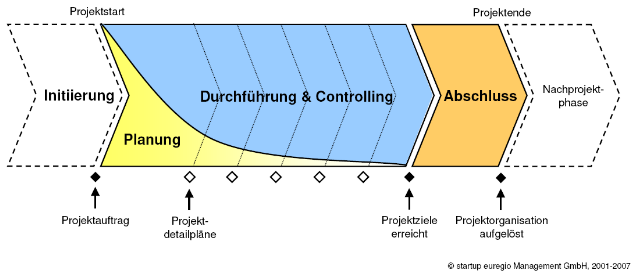
\includegraphics[width=1.0\textwidth]{images/pm-prozess}
		\end{center}

	\end{frame}

	\begin{frame}{Intro - Projektbeteiligte}
	
		\begin{itemize}
			\item{Projektmitarbeiter}
			\item{Projektleiter}
			\item{Projektmanagement}
			\item{Stakeholder}
		\end{itemize}

	\end{frame}
	
	\thispagestyle{empty}
	\frame{\centering{\textbf{Welche Faktoren beeinflussen den Projekterfolg?}}}
	
	\begin{frame}{Faktoren für Projekt(-miss-)erfolg}
		
		Eine Studie der GPM: Erfolg und Scheitern von 2008 erhob Daten aus: 
		\begin{itemize}
			\item{Befragung von 79 Unternehmen, mit hohem Anteil aus Mobilindustrie, Consulting, IT, Versicherung u. Bank }
			\item{überweigend Organisationen mit mehr als 1000 Mitarbeitern}
			\item{Erhebungsmethodik: über 30 Fragen an erfolgreiche und gescheiterte Projekte; jede Frage konnte dabei mit 1 (''trifft garnicht zu") und 5 (''trifft voll zu") beantwortet werden; Durchschnittswert einer Frage wurde erfolgreichem Projekt und gescheiterten Projekt gegenübergestellt}
		\end{itemize}

	\end{frame}

	\begin{frame}{Faktoren für Projekt(-miss-)erfolg 2}
	Ergebnis der Studie:
		\begin{center}
			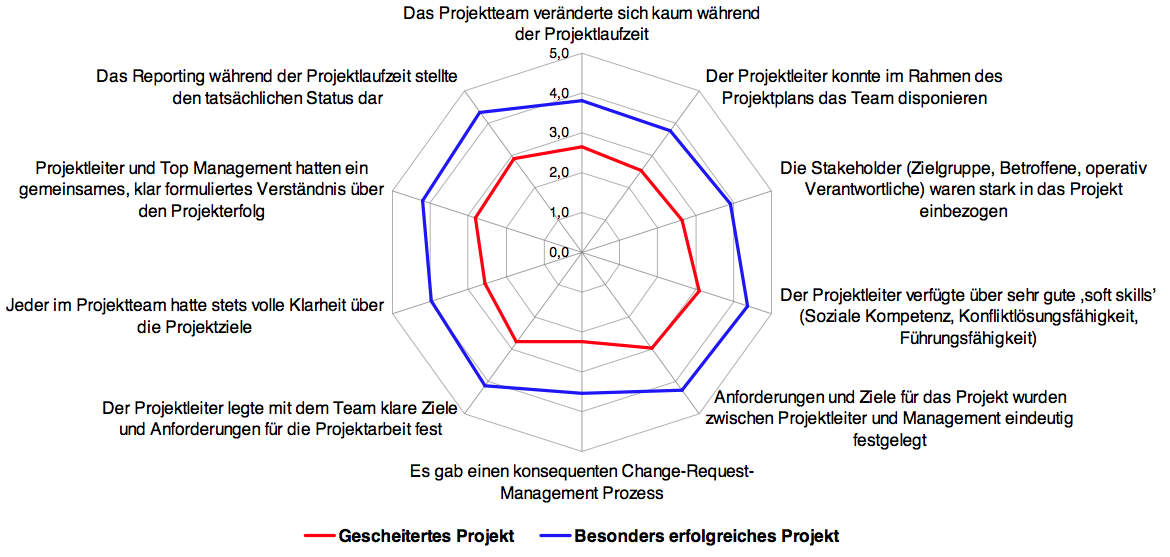
\includegraphics[width=1\textwidth]{images/studie_erfolgsfaktoren}
		\end{center}

	\end{frame}

	\begin{frame}{Faktoren für Projekt(-miss-)erfolg 3}
		Nach Gruppierung der Antworten, wurden folgende Top-5 Probleme festgestellt:
		\begin{itemize}
			\item{Kommunikation}
			\item{Unklare Ziele}
			\item{Position des Projektleiters}
			\item{PM-Prozesse}
			\item{Teambesetzung}
		\end{itemize}

	\end{frame}
	
%	\begin{frame}{Faktoren für Projekt(-miss-)erfolg 3}
%		Vorstellung von drei aus fünf: 
%		\begin{itemize}
%			\item{\textbf{Kommunikation}}
%			\item{Klare Ziele}
%			\item{\textbf{Position des Projektleiters}}
%			\item{PM-Prozesse}
%			\item{\textbf{Teambesetzung}}
%		\end{itemize}
%	\end{frame}

	% Mark: Problem Kommunikation
	\thispagestyle{empty}
	\begin{frame}
		''Der Widerspruch zwischen dem, was gesagt wird, und dem, was gemeint ist, ist sehr groß. Man muß ihn herausfinden.'' \\ 
		- \textit{Friedrich Eberling (Vorstandsvorsitzender Braun und Brunnen AG)}
	\end{frame}

	\begin{frame}{Kommunikationsprobleme}
		% TODO: Probleme listen
		\begin{itemize}
			\item{es wird zu wenig kommuniziert}
			\item{es wird zuviel kommuniziert}
			\item{Fachsprache vs. Fachsprache}
			\item{Sprachunterschiede in interkulturellen Projekten}
			\item{Dokumentation}
			\item{Informationen freigeben oder behalten}
			\item{Interessenskonflikte}
		\end{itemize}
	\end{frame}
	
	% TODO: Beispiel 
	\begin{frame}{Kommunikationsprobleme - Beispiel}
		
	\end{frame}
	
	\begin{frame}{Kommunikationsprobleme - Tipps}
		\begin{itemize}
			\item{zuviel Kommunikation ist besser als zuwenig}
			\item{regelmäßige Treffen mit allen Projektbeteiligten}
			\item{einrichten eines Besprechungsmanagements}
			\item{Dokumentationskriterien festlegen}
			\item{}
		\end{itemize}
	\end{frame}

	% TODO: Quizfrage
	\begin{frame}{Kommunikationsprobleme - Quizfrage}
		\textbf{Wie kann Kommunikation in einem Projekt verbessert werden?} (Diskussionsansatz)
	\end{frame}

	\begin{frame}{Kommunikationsprobleme - Quizfrage}
		\textbf{Wie kann Kommunikation in einem Projekt verbessert werden?} \\
		\begin{itemize}
			\item{Vertrauen schaffen}
			\item{Konfliktmanagement}
			\item{}
		\end{itemize}

	\end{frame}

	% Mark: Problem Projektziele
	\thispagestyle{empty}
	\begin{frame}
		''Fleiß für die falschen Ziele ist noch schädlicher als Faulheit für die richtigen.'' \\
		- \textit{Peter Bamm (1897 - 1975, dt. Arzt u. Schriftsteller)}
	\end{frame}

	
	\begin{frame}{Problem der unklaren Projektziele}
		Unklare Ziele führen zu:
		\begin{itemize}
			\item{hohen Projektkosten}
			\item{Verschwendung von Projektressourcen}
			\item{noch mehr Kommunikation}
			\item{Verschiebung des Zeitplans}
		\end{itemize}

	\end{frame}

	\begin{frame}{Problem der unklaren Projektziele - Beispiel}
		Gegeben sei ein Projekt zur Weiterentwicklung eines Ticket-Systems für ein Software-Produkt. Folgende Zielsetzung kann aufgestellt werden: \\
		\framebox{
			\colorbox{red!20}{
				\parbox{0.4\textwidth}{
Support-Request-Response-Zeiten\\ 
verbessern
				}
			}
		}
\framebox{
	\colorbox{green!20}{
		\parbox{0.4\textwidth}{

Support-Request-Response-Zeiten\\ 
um 10 \% bis 31.12.2013 reduzieren. 
		}
	}
}

		
	\end{frame}

	\begin{frame}{Projektziele richtig definieren}
		\begin{itemize}
			\item{Mehrere kleinere genau defineirte Projektziele}
			\item{Meilensteine}
			\item{SMART}
		\end{itemize}
	\end{frame}

	\begin{frame}{Unklare Projektziele - Quizfrage}
		Gegeben sei folgendes Projektziel:\\
		\textbf{Für das Projekt soll eine Versionsverwaltung verwendet werden.} \\
		Schlecht formuliertes Ziel? \\
	\end{frame}

	\begin{frame}{Unklare Projektziele - Quizfrage}
		Gegeben sei folgendes Projektziel:\\
		\textbf{Für das Projekt soll eine Versionsverwaltung verwendet werden.} \\
		Schlecht formuliertes Ziel? \\
		Antwort: \\
		Ja, Präzisision der Aufgabe nötig: Welche Versionsverwaltung? Bis wann? Extern? Intern? ... 
	\end{frame}

	\thispagestyle{empty}
	\begin{frame}
		''Führen ist eine besondere Kategorie des Dienens.'' - Hans L. Merkle (1913-2000), dt. Topmanager, 1963-84 Vors. d. GF Bosch AG
	\end{frame}

	\begin{frame}{Position des Projektleiters}
		\begin{itemize}
			\item{Soft Skills}
			\item{Erfahrung}
			\item{Motivation}
		\end{itemize}

		Problem, wenn der Projektleiter
		\begin{itemize}
			\item{zu hoch}
			\item{zu niedrig} 
		\end{itemize}
		angesiedelt ist.
		
	\end{frame}

	\begin{frame}{Position des Projektleiters - Beispiel}
		Jetzt kommt ein Erfahrungsbericht!
	\end{frame}

	\begin{frame}{Projektleiter - Tipps}
		\begin{itemize}
			\item{Anreize schaffen}
			\item{PL und PM integrieren}
			\item{kommunizieren, kommunizieren, kommunizieren}
			\item{Vertrauen aufbauen}
			\item{Einzelgespräche mit Projektmitarbeitern}
		\end{itemize}

	\end{frame}


	\thispagestyle{empty}
	\begin{frame}
		
		''Ein Prozess ist eine Maschinerie, die man als Schwein betritt und als Wurst verlässt.''  - Ambrose Bierce
		
	\end{frame}
	
	\begin{frame}{Probleme in PM-Prozessen}
		\begin{itemize}
			\item{Definition (nach DIN): Prozess zur Planung, Überwachung und Steuerung von Projektphasen}
			\item{iterativ und fordert Zeit}
			\item{Projektmanagement wird als ''Methode'' gesehen, nicht als Organisationsansatz}
			\item{Zeitprobleme}
		\end{itemize}
	
	\end{frame}
	
	\thispagestyle{empty}
	\begin{frame}
		''Teamwork = Wenn fünf Leute für etwas bezahlt werden, was vier billiger tun könnten, wenn sie nur zu dritt wären und zwei davon verhindert.''\\
- \textit{Charles Saunders}
	\end{frame}

	
	\begin{frame}{Probleme im Team}
		\begin{itemize}
			\item{Teamgröße}
			\item{Fluktuation}
			\item{Motivation}
			\item{''Ich Kann`s am besten''}
			\item{Interessenskonflikte}
		\end{itemize}
	\end{frame}

	\begin{frame}{Probleme im Team - Beispiel}
		Jetzt kommt noch ein Erfahrungsbericht!	
	\end{frame}

	\begin{frame}{Fazit}
		Studie der GPM (wie auch andere) führen zu folgendem Ergebnis für erfolgreiches Projektmanagement:
		\begin{itemize}
			\item{Projektleiter in die Projektorganisation integrieren}
			\item{Klare Ziele}
			\item{Gute Kommunikation}
			\item{Verständnis über PM als Organisationssturktur im Unternehmen}
		\end{itemize}
	\end{frame}
	
	\begin{frame}{Quellen}
		
	\end{frame}

	\begin{frame}{FKK}
		\begin{itemize}
			\item{Fragen?}
			\item{Kommentare?}
			\item{Kritiken?}
		\end{itemize}

	\end{frame}

	\thispagestyle{empty}
	\begin{frame}
		\begin{center}
			
\includegraphics[width=0.15\textwidth]{images/github} \\
			Fork me at \\
			https://github.com/olivererxleben/projectprobs
		\end{center}
	\end{frame}


\end{document}